\subsection{Path Generation}\label{subsec:prob2.1}
\begin{wrapfigure}{r}{0.5 \textwidth}
    \begin{center}
     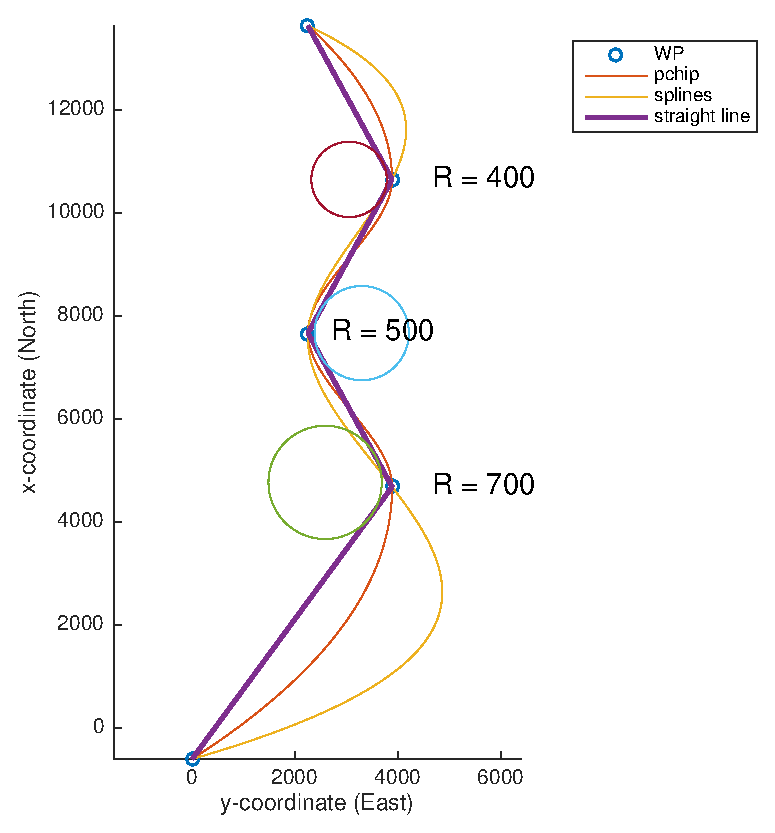
\includegraphics[width= 0.7 \textwidth]{task2.1/Task2_1}
     \end{center}
    \caption{Different trajectories}
    \label{fig:task2_1}
\end{wrapfigure}
We can see from figure \ref{fig:task2_1} that both methods based on continuous interpolation ("Piecewise Cubic Hermite Interpolating Polynomial" and "Cubic spline data interpolation") are very smooth, but they are more off-track than on-track. The pice-wise continuous interpolation are the crudest method of them all, since it in no way takes in to consideration the dynamics of the ship. The combination of circles and straight lines may look like the obvious best solution, but it does have a step in yaw rate ($r$), which means that the ship will not be able to follow the circle exactly while turning. Beside that, the lines and circles makes an excellent path for a ship to follow since it reduces the amount of time the ships actively uses it´s rudder, and therefore minimizes the drag on the ship. The turning radius set in the last method would be selected equal or larger to the ships turning radius. Preferably set it large enough to not loose to much speed, and small enough to not collide with someone/something. The nice about these turning radius, is that they can be adapted to the situation.

